%!TEX TS-program = xelatex
% !TeX spellcheck = it_IT 
\documentclass[11pt]{friggeri-cv}

\begin{document}
\header{Gessica Trivelli}{Ostetrica}

% In the aside, each new line forces a line break
\begin{aside}
  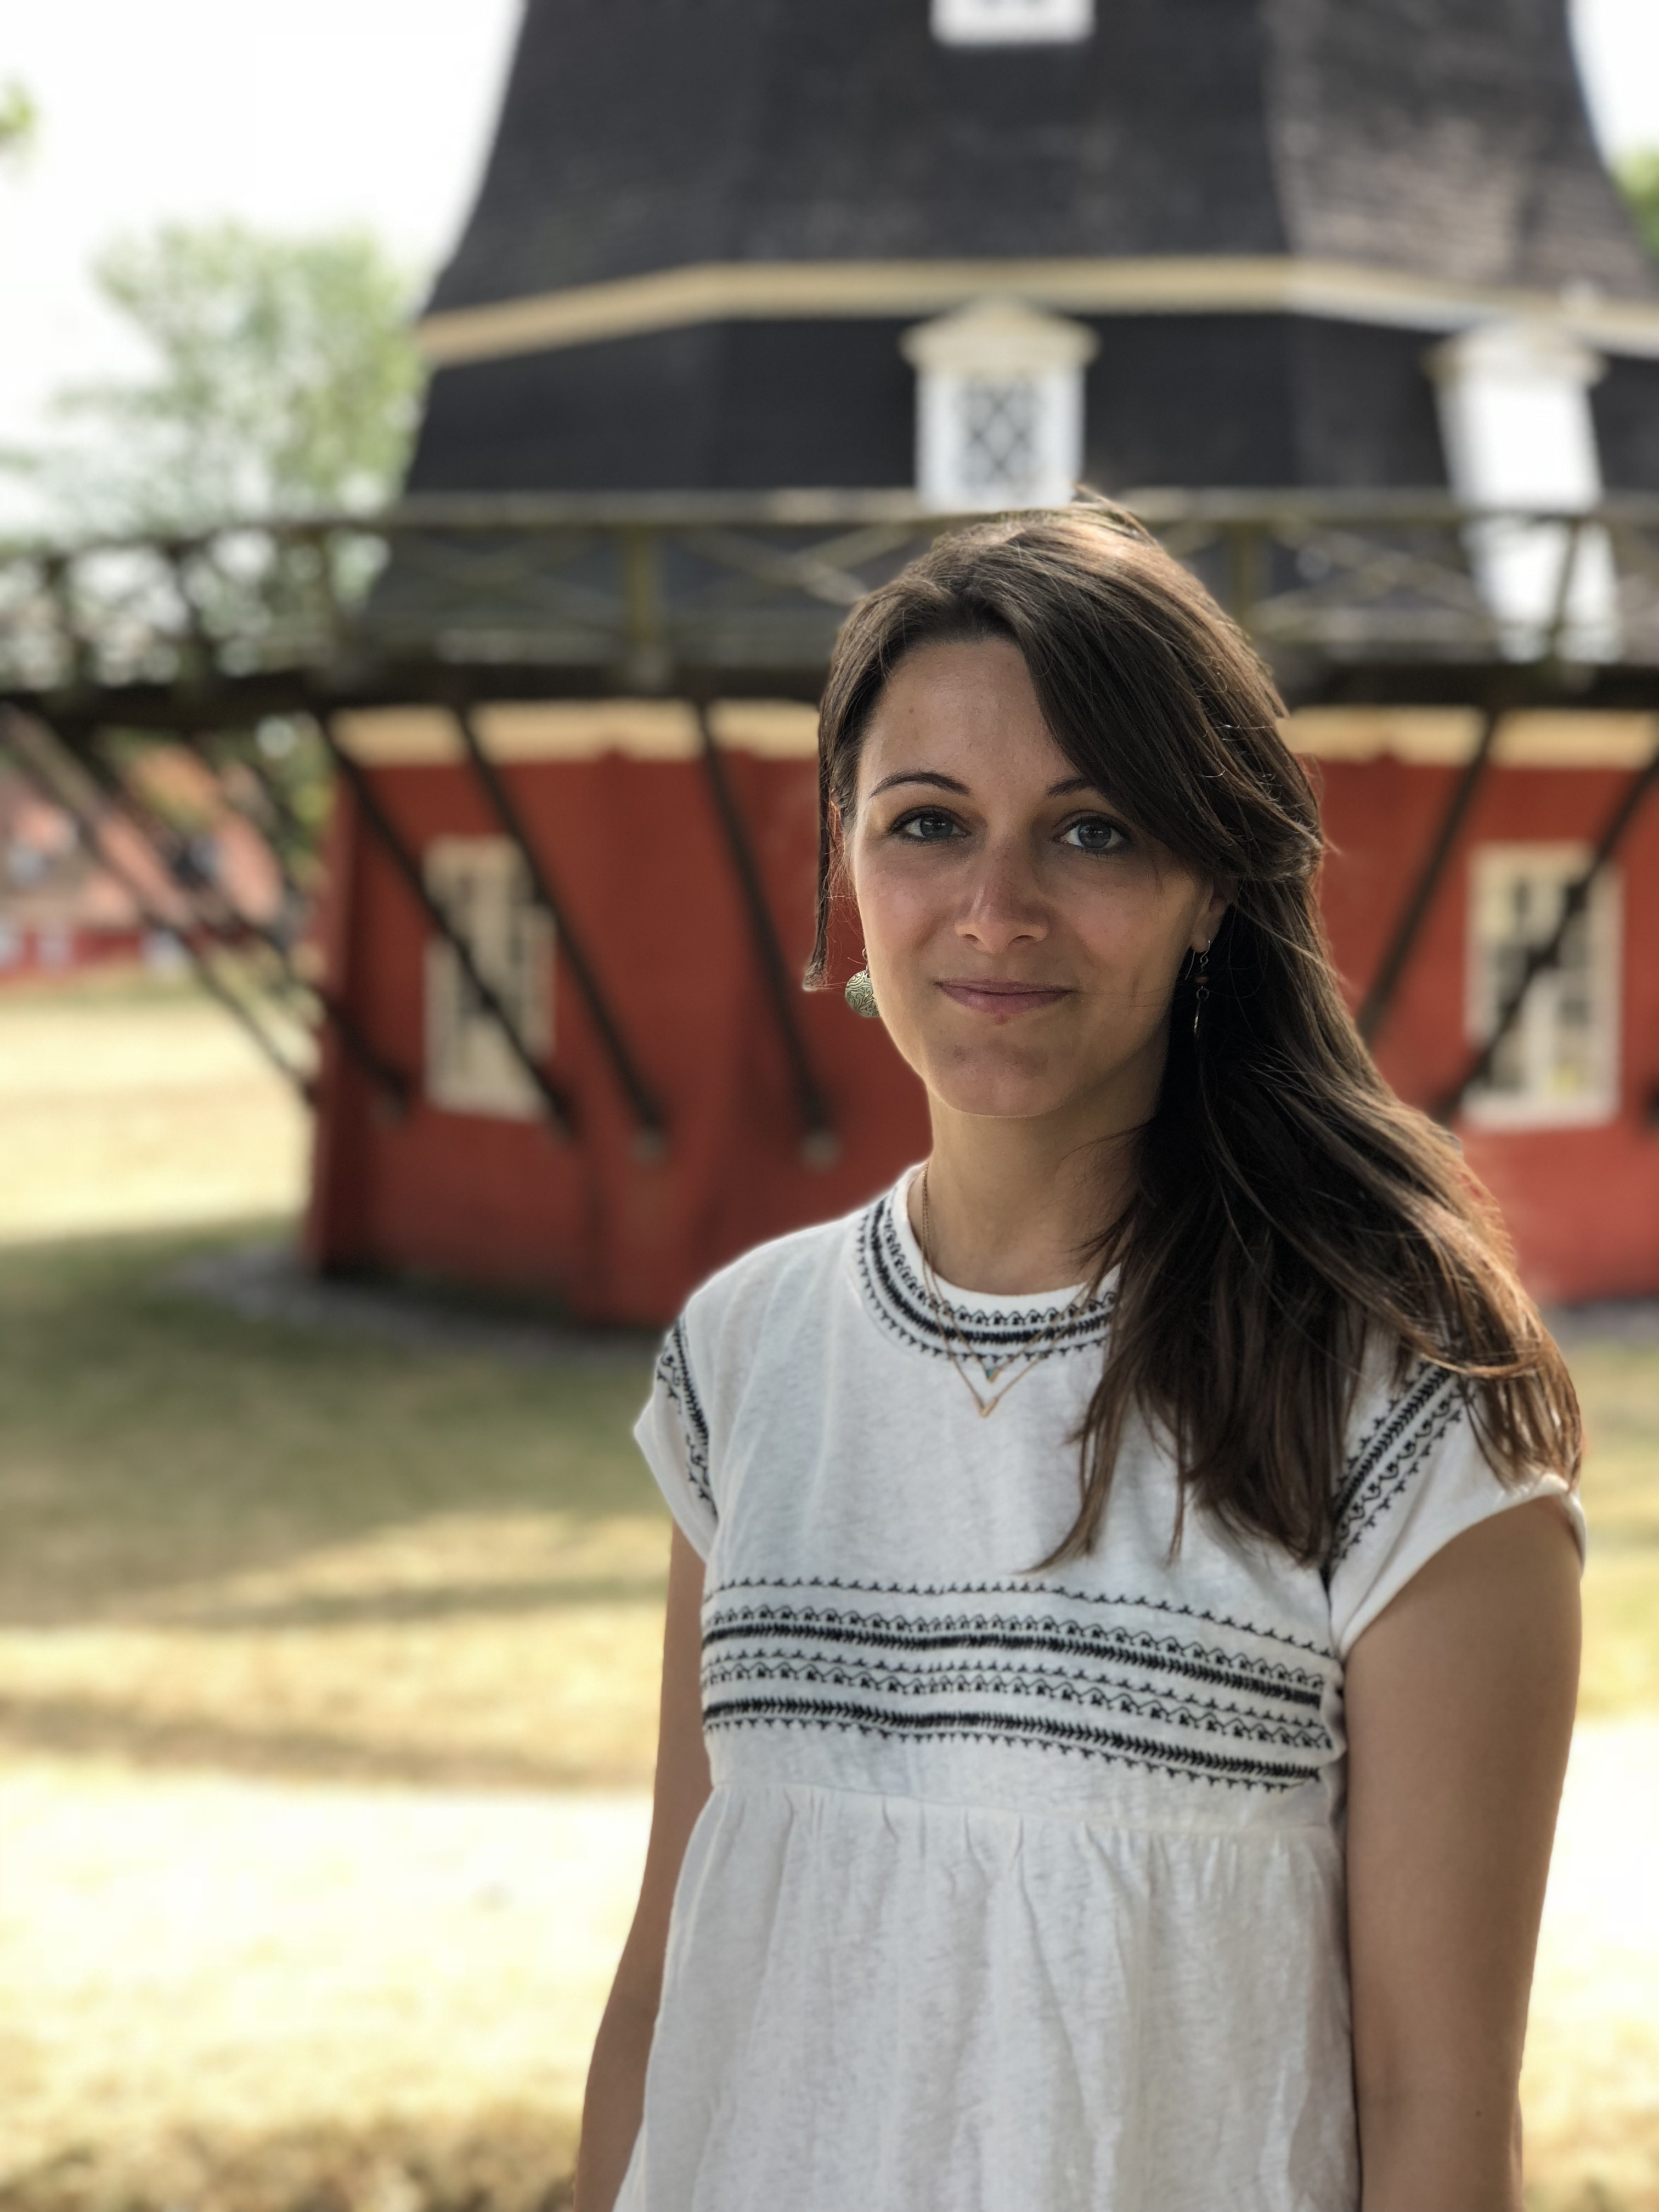
\includegraphics[width=0.95\columnwidth]{img/IMG_2838}
  \section{Skype}{\footnotesize{
    gessica.trivelli@gmail.com}}
  \section{Mail}{\footnotesize{
    \href{mailto:gessica.trivelli@gmail.com}{gessica.trivelli@gmail.com}}}
  \section{Informazioni Personali}\footnotesize{
    \textbf{Nazionalita'}: 
    Italiana
    \textbf{Data di Nascita}: 14/04/1991}
\end{aside}

\vspace{-10pt}
\section{Istruzione e Formazione}
\begin{entrylist}
  \entry
  {2017 - 2018}
  {Corso di Specializzazione}
  {\\Scuola Elementale di Arte Ostetrica, Firenze}
  {\emph{La salute pelvica nei cicli femminili: educazione, prevenzione, 
    rieducazione e trattamento delle disfunzioni perineali con approccio 
    ostetrica-specifico}. \\
    Corso di 50 crediti ECM - 194 ore.\\ 
    Titilo Tesi: \emph{Il prolasso degli organi pelvici: oltre l’intervento 
    chirurgico}.\\
  }

  \entry
  {2014 - 2017}
  {Laurea Magistrale in Scienze Infermieristiche e Ostetriche}
  {\\Universita' di Roma Tor Vergata}
  {Voto: 110/110 e Lode\\ Titolo Tesi Sperimentale: \emph{Conoscenze e 
    atteggiamenti delle mamme e delle ostetriche sul tema del clampaggio 
    tardivo del cordone ombelicale e donazione di sangue neonatale.} 
    \\Tirocinio di Ricerca svolto presso \textit{Istituto Superiore di Sanita' 
    di Roma, via Giano della Bella, n°34}.\\
  }
  
  \entry
  {2010 - 2014}
  {Laurea in Ostetricia}
  {\\Universita' di Roma Tor Vergata}
  {Voto: 110/110 e Lode\\
    Titolo Tesi Sperimentale: \emph{Indagine sul movimento libero e le 
    posizioni 
    antalgiche del travaglio e del parto: valutazione degli outcomes 
    materno-fetali.} \\
    Tirocinio Formativo svolto presso le seguenti strutture ospedaliere: 
    \textit{Policlinico Tor 
    Vergata}, \textit{Azienza Ospedaliera San Giovanni Addolorata}, 
    \textit{Ospedale Fatebenefratelli San Giovanni Calibita} e 
    \textit{Policlinico 
    Casilino}.\\
  }
  
  \entry
  {2005-2010}
  {Diploma di Liceo Scientifico}
  {\\Liceo Scientifico "A. Gentili", Sarnano (MC)}
  {\\}
\end{entrylist}

\vspace{-20pt}
\section{Esperienze Lavorative}
\begin{entrylist}
  \entry
  {04/2019\\Oggi}
  {Ostetrica}
  {\\Helios Klinik di Titisee-Neustadt, Germania}
  {Sala Parto.}
  \\ \\ \\
  \entry
  {07/2017\\11/2018}
  {Ostetrica}
  {\\Coombe Women and Infants University Hospital di Dublino, Irlanda}
  {Ambulatorio Ostetrico-Ginecologico.\\
    Reparto di Ostetricia e Patologia Ostetrica.\\
    Pronto Soccorso Ostetrico.}
\end{entrylist}
\vspace{-10pt}
\begin{aside}
  \section{IT Skills}
  \textbf{Office}
\includegraphics[scale=0.40]{img/5stars.png}
  \textbf{Epi-Info}
\includegraphics[scale=0.40]{img/3stars.png}
  \textbf{Pubmed}
\includegraphics[scale=0.40]{img/5stars.png}
  \section{Abilita' e Competenze Tecniche}\footnotesize{
    Problem solving 
    ~
    Utilizzo di modelli didattici innovativi
    ~
    Formazione degli adulti
    ~
    Pianificazione, implementazione e valutazione in ambito clinico, organizzativo e 
    pedagogico 
    ~
    Ricerca qualitativa e quantitativa in ambito clinico, organizzativo e pedagogico 
    ~
    Valutazione del servizio sanitario (e.g. qualita', pertinenza, sicurezza e 
    costo)}
  \section{Competenze Relazionali}\footnotesize{
  Assistenza incentrata sulla donna, promuovendo l'informazione e la 
  liberta' di scelta, attraverso competenze quali, counselling, empatia e 
  ascolto attivo.}
\end{aside}


\section{Certificazioni}
\begin{entrylist}
  \entry
    {2018}
    {BLS provider - American Heart Association}
    {\\Center for Midwifery Education, Dublino - Irish Heart Foundation}
    {\vspace{-10pt}}
  \entry
    {2018}
    {K2MS Perinatal Training Programme (PTP).}
    {\\K2MS, Dublino}
    {Fetal monitoring and maternity crisis management training}
  \entry
    {2018}
    {Breastfeeding Refresher Programme}
    {\\Center for Midwifery Education, Dublino}
    {\vspace{-10pt}}
  \entry
    {2018}
    {Diabetes in Pregnancy Update}
    {\\Center for Midwifery Education, Dublino}
    {\vspace{-10pt}}
  \entry
    {2018}
    {Preceptorship Programme for Midwives and Nurses}
    {\\Center for Midwifery Education, Dublino}
    {\vspace{-10pt}}
  \entry
    {2018}
    {Water Immersion for Labour and Birth}
    {\\Center for Midwifery Education, Dublino}
    {\vspace{-10pt}}
  \entry
    {2017}
    {Haemovigilance and Infection Control}
    {\\Center for Midwifery Education, Dublino}
    {\vspace{-10pt}}
  \entry
    {2016}
    {Emergenze del parto extra-ospedaliero}
    {\\CreAttivaMente Ostetriche, Roma}
    {Corso di 16 con uso di simulatore.}
  \entry
    {2015}
    {Competenze avanzate per il sostegno dell’allattamento al seno.}
    {\\CreAttivaMente Ostetriche, Roma }
    {Corso di 16 ore.}
  \entry
    {2014}
    {Allattamento al seno: corso pratico di counselling.}
    {\\Tor Vergata, Universita' di Roma Tor Vergata}
    {Corso di 40 ore.}
\end{entrylist}

\vspace{-10pt}
\section{Competenze Linguistiche}
\begin{table*}[!h]
  \centering
  \renewcommand{\arraystretch}{1.45}
  \begin{tabular}{ p{3cm} p{3cm} p{3cm} p{3cm} }
    \hline
    & \textbf{Scritto}  & \textbf{Parlato} & \textbf{Ascolto}     \\     \hline
    \textbf{Italiano:}  & \multicolumn{3}{c}{Madrelingua}         \\
    \textbf{Inglese:}   & C1 & C1 & C1                            \\ 
    \textbf{Tedesco:}   & B2 & B2 & B2                            \\ 
    \textbf{Francese:}  & A1 & A1 & A2                            \\    \hline
  \end{tabular}
\end{table*}

\newpage
\section{Riconoscimenti}
\begin{entrylist}
  \entry
    {2016}
    {Borsa di Tutoraggio}
    {\\Universita' di Roma Tor Vergata}
    {250 ore}
  \entry
    {2013}
    {Borsa di Collaborazione}
    {\\Universita' di Roma Tor Vergata}
    {150 ore}
\end{entrylist}

\vspace{-10pt}
\section{Albo Professionale}
\begin{itemize}
  \item[--] Iscritta al Collegio delle Ostetriche di Roma in posizione 
  n°2640 in data 25/02/2015.
  \item[--] Iscritta al \emph{Land Baden-W{\"u}rttenberg 
  Regierungspr{\"a}sidium Stuttgart} in data 11/07/2019.
\end{itemize}

\vspace{75pt}
\footnotesize La sottoscritta è a conoscenza che, ai sensi dell’art. 26 della legge 
15/68, le dichiarazioni mendaci, la falsità negli atti e l’uso di
atti falsi sono puniti ai sensi del codice penale e delle leggi speciali. Inoltre, il 
sottoscritto autorizza al trattamento dei dati
personali, secondo quanto previsto dalla Legge 675/96 del 31 dicembre 1996.

\vspace{75pt}
\begin{flushleft}
\large\emph{Roma, 23 Agosto 2019}
\end{flushleft}
\begin{flushright}
\large\emph{Gessica Trivelli}
\end{flushright}

\end{document}

